\chapter{Implementación del sistema operativo}

Una vez que sabemos las decisiones tomadas y las tecnologías utilizadas, pasemos a estudiar cada una de las soluciones implementadas en confrontación con los requisitos estudiados.\\

Empezaremos por la puesta a punto del sistema de compilación y continuaremos con la configuración necesaria para el funcionamiento esperado del sistema operativo embebido. Dado el volumen del proyecto Yocto, describiremos solo parcialmente sus factores de configuración y el proceso de trabajo con él.

\section{Introducción y puesta a punto}

Como venimos mencionando a lo largo de la memoria, el proyecto Yocto se basa en la herramienta \textit{Open Embedded} y en el lenguaje de configuración \textit{Bitbake}, que permite ajustar desde parámetros del kernel hasta elegir paquetes que no se quiere sean instalados. Además, cabe destacar que se pueden compilar imágenes con Yocto de diversas formas, ya sea utilizando contenedores aislados (a modo de máquinas virtuales) o nuestro propio sistema Linux \textit{anfitrión}, como vemos en la documentación de inicio \cite{yocto-project-quick-start-build-system}. Por mi parte, siempre he preferido hacerlo en el propio sistema, dado que así se destinan a la compilación el 100\% de los recursos asignados disponibles y el tiempo de espera es menor.\\

Para el caso que nos ocupa, la versión utilizada del proyecto Yocto ha sido la \textbf{2.4} (de nombre \textit{Rocko}), dado que se trataba de la versión estable más avanzada en el momento del desarrollo.\\

La guía relativa a la puesta a punto la encontramos en el manual \textit{Quick Start} de la web \cite{yocto-project-quick-start} ya mencionado, y consiste principalmente en instalar las dependencias necesarias para nuestra distribución y clonar mediante \texttt{git} el núcleo del proyecto, llamado \textit{Poky}, con el comando siguiente (la opción \texttt{-b} elige la rama deseada):

\begin{center}
\texttt{git clone git://git.yoctoproject.org/poky -b rocko}
\end{center}

\subsection{Manipulación y compilación de prueba}

Una vez tenemos el núcleo, lo siguiente es empezar a configurar el resultado que queremos obtener. Si ejecutamos el comando \texttt{source oe-init-build-env}, se nos generará un directorio destino \textit{build} con una configuración de ejemplo para una máquina \textit{Qemu} de 32 bits.\\ 

La premisa de este tipo de sistemas de desarrollo es incluir lo mínimo para funcionar, y que sea el desarrollador quien elija las dependencias a incluir. Por tanto, aunque dicho archivo de configuración es grande, se trata de mucho código de ejemplo y comentarios de ayuda al recién llegado.\\

Aquí podemos elegir entre cambiar el dispositivo de destino y los paquetes a instalar, o seguir adelante con una imagen mínima de prueba de la siguiente forma:

\begin{center}
\texttt{bitbake core-image-minimal}
\end{center}

El nombre \texttt{core-image-minimal} hace referencia a la imagen de menor tamaño por defecto, por lo que para hacer pruebas es suficiente. \\

Habremos de esperar un tiempo de entre treinta minutos y dos horas aproximadamente a que se descarguen todos los paquetes necesarios y se compilen. Tras esto, se habrá generado un archivo de imagen con extensión \textit{.sdimg} en el directorio \textit{./build/tmp/deploy/images/raspberrypi3/}.\\

Podremos \textit{quemar} (o instalar) esta imagen en una tarjeta de memoria con la conocida utilidad \textit{dd}, presente en cualquier sistema GNU/Linux, siendo \texttt{/dev/sdX} el dispositivo referente a la tarjeta de memoria:\\

\texttt{sudo dd if=core-image-minimal-raspberrypi3.sdimg of=/dev/sdX}\\

Acto seguido podremos insertar la tarjeta de memoria en la placa y encenderla para entrar en el sistema.

\subsection{Variables de configuración del sistema}

La sintaxis de configuración es sencilla, y sigue la forma: 

\begin{center}
	\texttt{PARÁMETRO\_CONFIGURACIÓN = "valor deseado"}
\end{center}

En el directorio \textit{build} antes creado, podremos ir incorporando configuración al archivo \textit{conf/local.conf} con dicha sintaxis de la herramienta \textit{Bitbake} para instalar/borrar paquetes del dispositivo.\\

La sintaxis de código para añadir dependencias sería la siguiente (hemos de añadir esta línea al archivo \textit{conf/local.conf} mencionado):

\begin{center}
\texttt{IMAGE\_INSTALL\_append = `` <paquete1> <paquete2> ...''}
\end{center}

Si quisiéramos eliminar alguno de los paquetes incluidos por alguna librería necesaria, es tan fácil como sustituir \texttt{append} por \texttt{remove}.\\

Por otro lado, si profundizamos en los archivos de configuración descargados de cualquiera de los layers, encontramos en alguna ocasión configuración de la forma:

\begin{center}
\texttt{VARIABLE ?= "valor"}
\end{center}

Cuando un símbolo de interrogación acompaña a esta variable, significa que es un \textbf{valor por defecto}, fácilmente anulable por una asignación sin dicho símbolo en cualquier parte.\\

Por ejemplo, en la configuración por defecto, el dispositivo por destino se muestra tal que así:

\begin{center}
\texttt{MACHINE ?= "qemux86"}
\end{center}

En nuestro caso, borraremos la interrogación y escribiremos ``raspberrypi3'' entre comillas, dado que es nuestro dispositivo elegido (podemos consultar el listado completo en \href{http://layers.openembedded.org/layerindex/branch/master/machines/?q=&browse=1}{OpenEmbedded Layer Index}, junto con los layers necesarios para cada máquina).\\

\subsection{Layers y librerías}

Por otro lado, la forma de reutilizar librerías y capas ya existentes es sencilla. Podemos encontrar la lista completa de capas y paquetes pertenecientes a éstas en la referencia \cite{yocto-layers-list}. Para empezar basta con descargarlas (también mediante \texttt{git}) en el directorio raíz del sistema de compilación. Acto seguido, añadimos una línea en el fichero \texttt{./build/conf/bblayers.conf} con la ruta a la librería descargada. [\textit{bblayers} toma su nombre por \textit{Bitbake Layers}.] Hecho esto, el comando \texttt{bitbake} detectará todos los paquetes y dependencias que tenemos importados en el sistema, viéndose esto reflejado en cada compilación.\\

En la web antes mencionada, \url{https://layers.openembedded.org}, dentro de la sección \textbf{\textit{Recipes}} podemos buscar paquetes que nos interesen, dando con la(s) capa(s) que los incluyen. Por ejemplo, si quisiéramos utilizar \textit{PSplash}, una herramienta para imprimir imágenes de carga embebidas, obtendríamos lo siguiente:

\begin{figure}[H]
	\centering
	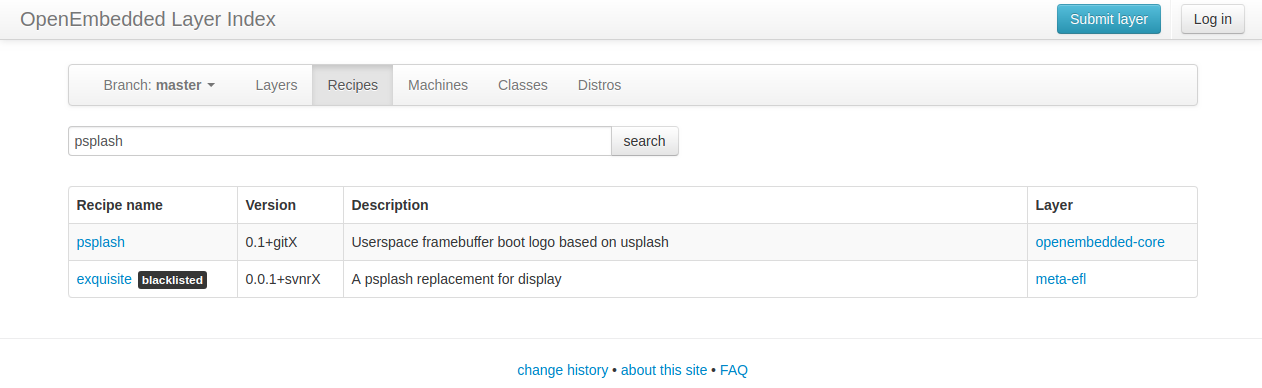
\includegraphics[width=\linewidth]{imagenes/yocto-recipe-search-example.png}
	\caption{Ejemplo de búsqueda en las recetas de OpenEmbedded [13/06/2018]}
	\label{yocto-recipe-search-example}
\end{figure}

Como vemos, los resultados vienen compuestos del nombre de los paquetes, las versiones (para filtrar cuando existen varias del mismo), una descripción inteligible y el layer donde encontrarlo. Si hacemos click en el nombre del layer, veremos una descripción de dicha capa y la dirección del repositorio donde se aloja (y que habremos de clonar).\\

\subsubsection{Layer propio}

Como aconsejan en la propia documentación de Yocto, una vez que queremos pasar de hacer pruebas a confeccionar nuestro producto, lo idóneo es \textbf{crear un \textit{layer} propio} en el que alojar la configuración de forma aislada. Por ejemplo, en nuestro caso la capa usada recibe el nombre de \texttt{meta-dynasystem} y da nombre a este proyecto.\\

Los pasos para crear un layer, descritos en la propia \textit{Wiki} de Yocto \cite{wiki-yocto-own-layer}, son sencillos. El proceso consiste básicamente en generar un par de carpetas y un archivo de configuración común al layer (llamado \textit{layer.conf}), describiendo las rutas internas a la capa y la prioridad de sus paquetes con respecto a los de otras.\\

Por otro lado, debemos saber que dentro de cada layer existirán distintos directorios 

\begin{itemize}
	\item \textbf{Configuración propia del layer \textit{(/conf)}}: el archivo necesario se aloja en la ruta antes mencionada \texttt{./conf/layer.conf}.
	\item \textbf{Ficheros de clases \textit{(/classes)}}: las clases representan comportamientos específicos que pueden heredar las imágenes de sistema. Tienen extensión \texttt{.bbclass}.
	\item \textbf{Recetas de paquetes de todo tipo \textit{(/recipes-X)}}: siendo ``X'' variable y reflejando el tipo de las recetas que se usan. Por ejemplo, los paquetes importantes o las imágenes suelen ser incluidas en una carpeta llamada \textbf{\textit{recipes-core}}; o las recetas relacionadas con Mender se agrupan en la carpeta \textbf{\textit{recipes-mender}}.
\end{itemize}

Dentro de estas carpetas de recetas encontraremos un directorio por cada paquete de la categoría. Comentemos esto en el siguiente apartado.\\

\subsection{Paquetes, configuración y parches}

Como hemos dicho anteriormente, encontramos una carpeta para cada paquete existente, con el mismo nombre del paquete. De forma interna a esta, podremos distinguir varios subdirectorios y archivos:

\begin{itemize}
	\item \textbf{Archivos a incluir en el sistema \textit{(/files)}}: aquí se alojan ficheros de todo tipo que se quiere figuren en el sistema final asociados al paquete (scrips, documentos, etc.).
	\item \textbf{Parches por aplicar al paquete \textit{(/patches)}}: comentaremos su función de forma más extensa en esta sección más adelante.
	\item \textbf{Configuración adicional para el paquete \textit{(paquete\_\%.bbappend)}}: <paquete> se refiere al nombre, y ``\%'' simboliza el número de versión. En este archivo se hace referencia a los ficheros del directorio \textit{/files} y los parches de \textit{/patches} que se quieren tomar en consideración.
\end{itemize}

Para terminar con la introducción a Yocto, cabe destacar la importancia de \textbf{los parches} previamente mencionados (o \textit{patches} en inglés). Estos permitirán de una forma escalable y, sobre todo automatizada, modificar el comportamiento de las aplicaciones y programas libres ya presentes en los repositorios.\\

Para entender el funcionamiento de los parches, veamos antes los estados por los que pasa un paquete por compilar:

\begin{enumerate}
	\item Se descarga el código fuente de la aplicación. El repositorio desde el que se descarga vendrá especificado por el fichero \textbf{\textit{``receta.bb''}} propio del paquete. Por ejemplo, la receta del paquete PSplash \cite{yocto-recipe-psplash}. La variable que almacena el enlace se llama \texttt{SRC\_URI}.
	\item Los layers pueden aplicar configuración y parches al código descargado de otros layers, guardando estas modificaciones en archivos \textbf{\textit{``receta.bbappend''}}. Después del primer paso, para cada paquete se buscan todos los ficheros \textit{.bbappend} que le correspondan, y se aplican las modificaciones oportunas.
	\item Una vez aplicados todos los parches, se compila el código completo y se incluye para ser instalado en la imagen de destino.
\end{enumerate}

Esto representado en UML en forma de diagrama de estados sería tal que así:

\begin{figure}[H]
	\centering
	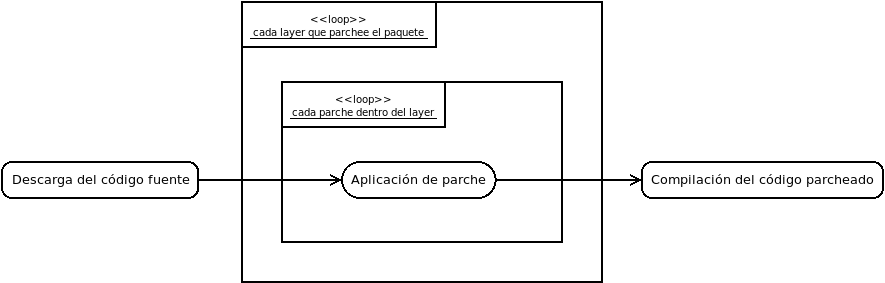
\includegraphics[width=\linewidth]{imagenes/statechart-parche.png}
	\caption{Diagrama de estados por los que pasa una dependencia en Open Embedded}
	\label{statechart-parche}
\end{figure}

\noindent\makebox[\linewidth]{\rule{\textwidth}{0.4pt}}\\

\subsubsection{Proceso de parcheo de paquetes}

Por otro lado, un recién llegado al proyecto podría pensar que la forma de redefinir comportamientos en paquetes ya existentes consiste en:

\begin{enumerate}
	\item Hacer en otro repositorio un \textit{fork} del programa en cuestión.
	\item Realizar las modificaciones pertinentes de forma aislada.
	\item Crear una receta en Yocto que obtenga el paquete desde el nuevo repositorio, con prioridad mayor al original.
\end{enumerate}

Yo mismo probé a hacerlo durante un tiempo, pero a pesar de que esto realmente puede llegar a ``funcionar'', es desacertado, pues además de ser lento y arduo no aporta escalabilidad ni automatización de ningún tipo.\\

La forma escalable de trabajar viene dada por \textbf{la herramienta \textit{devtool}}, que genera una copia local del código fuente del programa listo para que realicemos las modificaciones pertinentes. Además, nos permitirá realizar compilaciones utilizando esta versión temporal, para verificar el funcionamiento de los cambios añadidos. Encontramos la guía de estos pasos en la referencia \cite{wiki-yocto-patches}.\\

Ejecutamos \texttt{devtool nombre\_del\_paquete} y la herramienta descargará el código fuente, le serán aplicados todos los parches de las capas existentes por parte de \textit{bitbake}, y será generada una carpeta \texttt{./build/tmp/sources/nombre\_del\_paquete} con este código final.\\

Sobre el código de este directorio será sobre el que hagamos las modificaciones. Para probar estos cambios, bastará con compilar el paquete de forma aislada (\texttt{bitbake nombre\_del\_paquete}) y ejecutarlo.\\

\subsubsection{Inclusión de parches en layer propio}

Cuando terminemos con las pruebas y queramos guardar los cambios realizados, deberemos generar un archivo en forma de parche interpretable de forma automática por Bitbake, y que quede de forma persistente en nuestro propio layer.\\

Bitbake detectará automáticamente la existencia de estos parches y los aplicará al código fuente del programa antes de compilarlo e instalarlo en la imagen de destino. Para desarrollar sistemas con Yocto, es una de las mecánicas más usadas, ya que generalmente existen paquetes para casi cualquier necesidad que tengamos, pero siempre están abiertos a modificaciones más especiales.\\

El comando de generación de parches es simple y conocido, dado que no es específico de Bitbake sino de GNU/Linux. Para el caso de un parche a un paquete genérico, el comando tendría la siguiente estructura:\\

\textit{\textbf{git diff ./build/tmp/sources/<paquete>/<fichero\_modificado> \\./<layer\_propio>/recipes-<X>/patches/<paquete>.patch}}\\

\noindent\makebox[\linewidth]{\rule{\textwidth}{0.4pt}}\\

Una vez que tenemos el parche generado e importado en nuestro layer, necesitaremos hacer ver a la receta original del paquete parcheado la existencia de dichas modificaciones. Para ello crearemos una receta del tipo \textit{.bbappend} como las ya antes mencionadas, con el siguiente contenido:

\begin{lstlisting}
FILESEXTRAPATHS_prepend := "${THISDIR}/patches:"
\end{lstlisting}

Esto provocará que Bitbake automáticamente tenga en cuenta estos cambios y los incorpore sobre el código original del paquete.\\

Una vez hayamos hecho esto, podremos centrarnos en los paquetes utilizados y/o desarrollados para satisfacer las necesidades del producto.

\section{Desarrollo de los paquetes necesarios}

Una vez que tenemos una ligera idea de cómo funciona el entorno de trabajo de \textit{Open Embedded/Yocto Project} nos será más sencillo entender las soluciones implementadas para satisfacer los requisitos estudiados.\\

Empezaremos por generar una imagen para un sistema mínimo, sobre la que iremos añadiendo dependencias que satisfagan dichos requerimientos (funcionales o no funcionales).

\subsection{Sistema mínimo}

El archivo con la configuración final del sistema se encuentra en \texttt{dynasystem-image} \cite{dynasystem-image}, aunque la configuración mínima para funcionar sería, además de lo comentado en \textit{./build/conf/local.conf}, lo siguiente:\\

\texttt{\# dynasystem-image\\
inherit core-image\\
IMAGE\_INSTALL += "packagegroup-core-boot"\\
IMAGE\_FEATURES += "ssh-server-dropbear"}\\

-- El nombre \texttt{core-image} hace referencia a la clase mínima necesaria para cualquier imagen de Yocto.\\

-- Con la segunda línea hacemos referencia a todo el grupo de paquetes necesarios para arrancar una máquina con los paquetes mínimos necesarios.\\

-- Por último, instalamos la característica del servidor SSH para administrar de forma fácil el sistema.\\

Una vez que tenemos esta configuración guardada en el fichero \textit{./meta-dyna-system/recipes-core/images/dynasystem-image.bb}, basta con compilar la imagen con la orden: \texttt{bitbake dynasystem-image}.\\

En este punto la distribución no aporta gran cosa, ya que lo único que hace es cargar el kernel sin apenas programas instalados. Para dotarle de funcionalidades, necesitaremos ver la siguiente sección.

\subsection{Soluciones implementadas/usadas}

\texttt{POR EXPLICAR:\\
	- autologin\\
	- arranque silencioso (no terminal)\\
	- [seguridad] no entrada teclado\\
	- [seguridad] no ejecución sin aplicación (watcher)\\
	- [actualizaciones] salvar redes wifi\\
	- [app] ejecución de la aplicación embebida\\
	- [app] librerías de qt\\
	- [actualizaciones] actualizacion interna de la electronica\\
	- conectividad inalámbrica (wifi \& bluetooth)\\
	- soporte de audio\\
	- pantalla completa durante carga\\
	- ficheros. soporte para usb's (formatos ntfs, fat, exfat)\\
	- [actualizaciones] actualización a través de servidor\\
	- [actualizaciones] confirmación por parte del usuario}\\

\section{Integración con el gestor de actualizaciones}

Por explicar integración con Mender, paquetes necesarios, etc.

\newpage